\documentclass[a4paper,12pt,oneside]{book}

%------------------------------- Start of the Preable ------------------------------------------------
\usepackage[english]{babel}
\addto{\captionsenglish}{%
\renewcommand{\bibname}{References}
\renewcommand{\refname}{References}
}

\usepackage{blindtext}
\usepackage{minted}
\setcounter{secnumdepth}{3}

%\usepackage[none]{hyphenat}
\usepackage[parfill]{parskip}

\usepackage{hyperref}
\hypersetup{
    colorlinks=true,
    linkcolor=blue,
    filecolor=magenta,      
    urlcolor=cyan,
}

\urlstyle{same}
%use of package fancy header
\usepackage{fancyhdr}
\usepackage{fancyvrb}
\setlength\headheight{26pt}
\fancyhf{}
%\rhead{
\includegraphics[width=1cm]{logo}}
\lhead{\rightmark}
\rhead{
\includegraphics[width=1cm]{images/logo}}
\fancyfoot[RE, RO]{\thepage}
\fancyfoot[CE, CO]{\href{http://www.e-yantra.org}{www.e-yantra.org}}

\pagestyle{fancy}

%use of package for section title formatting
\usepackage{titlesec}
\titleformat{\chapter}
  {\Large\bfseries} % format
  {}                % label
  {0pt}             % sep
  {\huge}           % before-code
 
%use of package tcolorbox for colorful textbox
\usepackage[most]{tcolorbox}
\tcbset{colback=cyan!5!white,colframe=cyan!75!black,halign title = flush center}

\newtcolorbox{mybox}[1]{colback=cyan!5!white,
colframe=cyan!75!black,fonttitle=\bfseries,
title=\textbf{\Large{#1}}}

%use of package marginnote for notes in margin
\usepackage{marginnote}

%use of packgage watermark for pages
%\usepackage{draftwatermark}
%\SetWatermarkText{
\includegraphics{logo}}
\usepackage[scale=3.2,opacity=0.1,angle=0]{background}
\backgroundsetup{
contents={
\includegraphics{images/logo-med}}
}

%use of newcommand for keywords color
\usepackage{xcolor}
\newcommand{\keyword}[1]{\textcolor{red}{\textbf{#1}}}

%package for inserting pictures
\usepackage{graphicx}

%package for highlighting
\usepackage{color,soul}

%new command for table
\newcommand{\head}[1]{\textnormal{\textbf{#1}}}

\usepackage{dirtree}
\usepackage{siunitx}

\makeatletter
\global\let\tikz@ensure@dollar@catcode=\relax
\makeatother

\usepackage{textcomp}

%---------------------- End of the Preamble ---------------------------------------


\begin{document}

%---------------------Title Page------------------------------------------------
\begin{titlepage}
\raggedright
{\Large eYSIP 2017\\[1cm]}
{\Huge \scshape Tutorial on Interfacing a Wireless Joystick Controller for Quadcopters \\[.1in]}

\vfill

\begin{figure}[!htb]
\centering
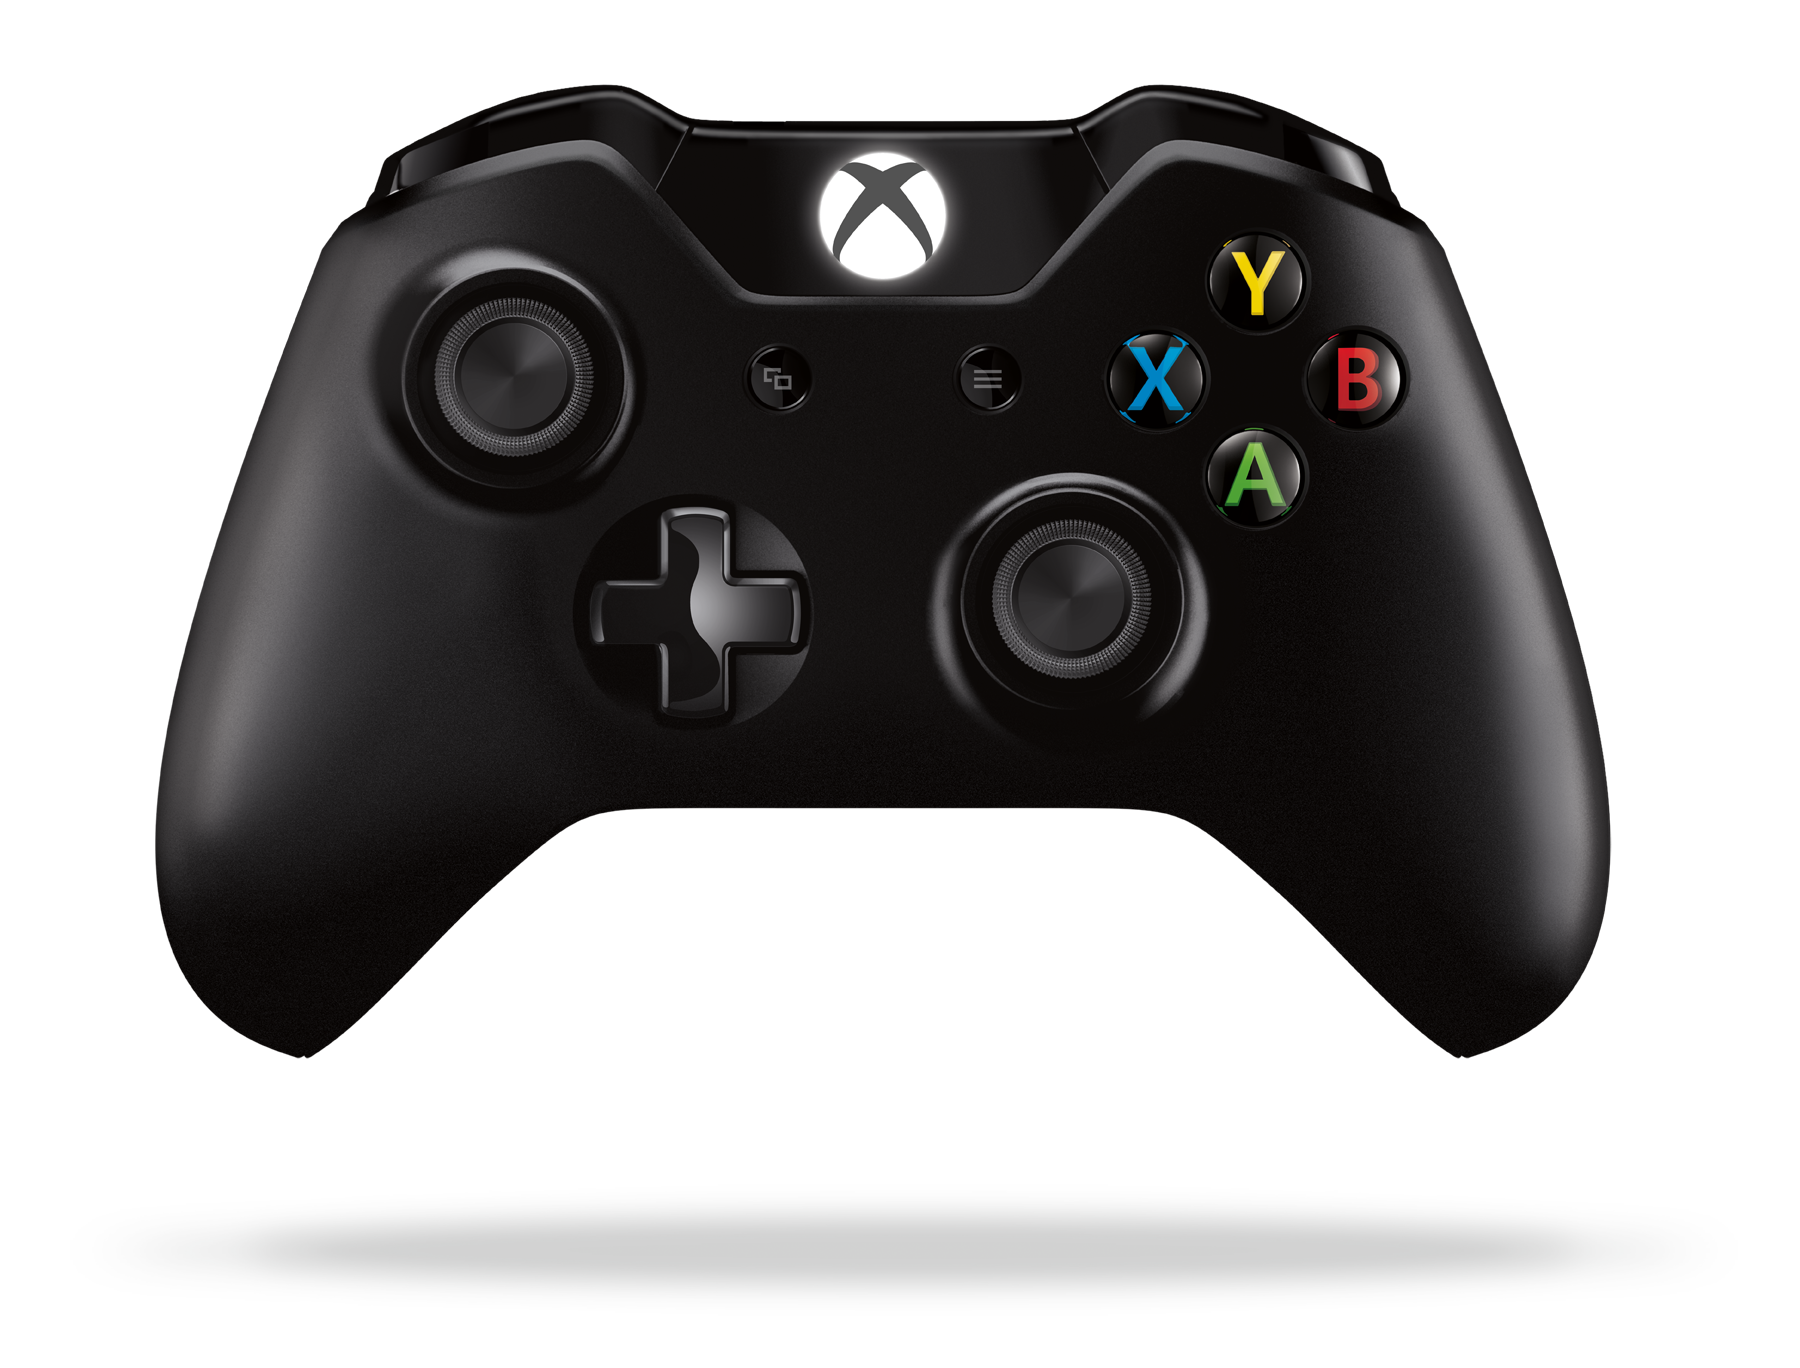
\includegraphics[width=0.85\textwidth]{images/xbox_one}
\\Xbox\textsuperscript{\textregistered} One Controller\cite{xbox}
\end{figure}

\vfill

\begin{flushright}
{\large Heethesh Vhavle \\}
{\large Sanam Shakya \\}
{\large Pushkar Raj \\}
\vspace{0.5cm}
{\large Duration of Internship: $ 22/05/2017-07/07/2017 $ \\}
\end{flushright}
\medskip

{\itshape 2017, e-Yantra Publication}
\end{titlepage}

%-------------------------------------------------------------------------------

%\tableofcontents
%\listoffigures

%-------------------------------------------------------------------------------

\chapter[Wireless Joystick Controller for Quadcopters]{Wireless Joystick Controller for Quadcopters}
\section{Introduction}
The project deals with the study of control algorithms and to develop a custom firmware for quadcopter (flight controller) on 32-bit micro-controllers. The flight controller is designed to control parameters such as the throttle, yaw, pitch and roll and consists of algorithms considering various motion and dynamics. One of the goals is to develop a wireless joystick controller for simple maneuvering of the quadcopter.\\ 

A very common method of piloting drones is by using a RC transmitter with 6-8 channels. In this project an USB-HID gamepad controller is interfaced with Python, which in turn transmits commands (MSP frames) to the quadcopter over Wi-Fi. Other than throttle and direction control for drones, there are certain other controls that must be provided to a pilot for a stable and safe flight. The list of controls implemented in the firmware is explained later.\\

In this project, the Xbox\textsuperscript{\textregistered} One Controller\cite{xbox} is used. this controller is a USB-HID Gamepad compliant device and is interfaced with Python with the help of \textit{pygame} module. The inputs from the controller are read, parsed, converted and then packed into MSP frames and sent to the quadcopter. Any other USB game controller can also be interfaced in the same way.\\

For communication with the drone and debugging purposes, it will be easier to do so with the help of serial communication port. But the PC is connected to the drone over Wi-Fi. A virtual COM port can be created with the help of softwares such as \href{https://www.eltima.com/products/serial-over-ethernet/}{Eltima Serial to Ethernet Connector} or \href{http://www.hw-group.com/products/hw_vsp/index_en.html}{HW Virtual Serial Port} which redirects the data from TCP/IP sockets to the COM ports.\\

\section{List of Controls}
\label{sec:loc}
Although flight planner/controller software such as MultiWii Conf exist, it is very difficult to pilot a drone using them, especially in emergency situations. Following is a list of controls implemented on the controller.\\

\begin{figure}[!htb]
\centering
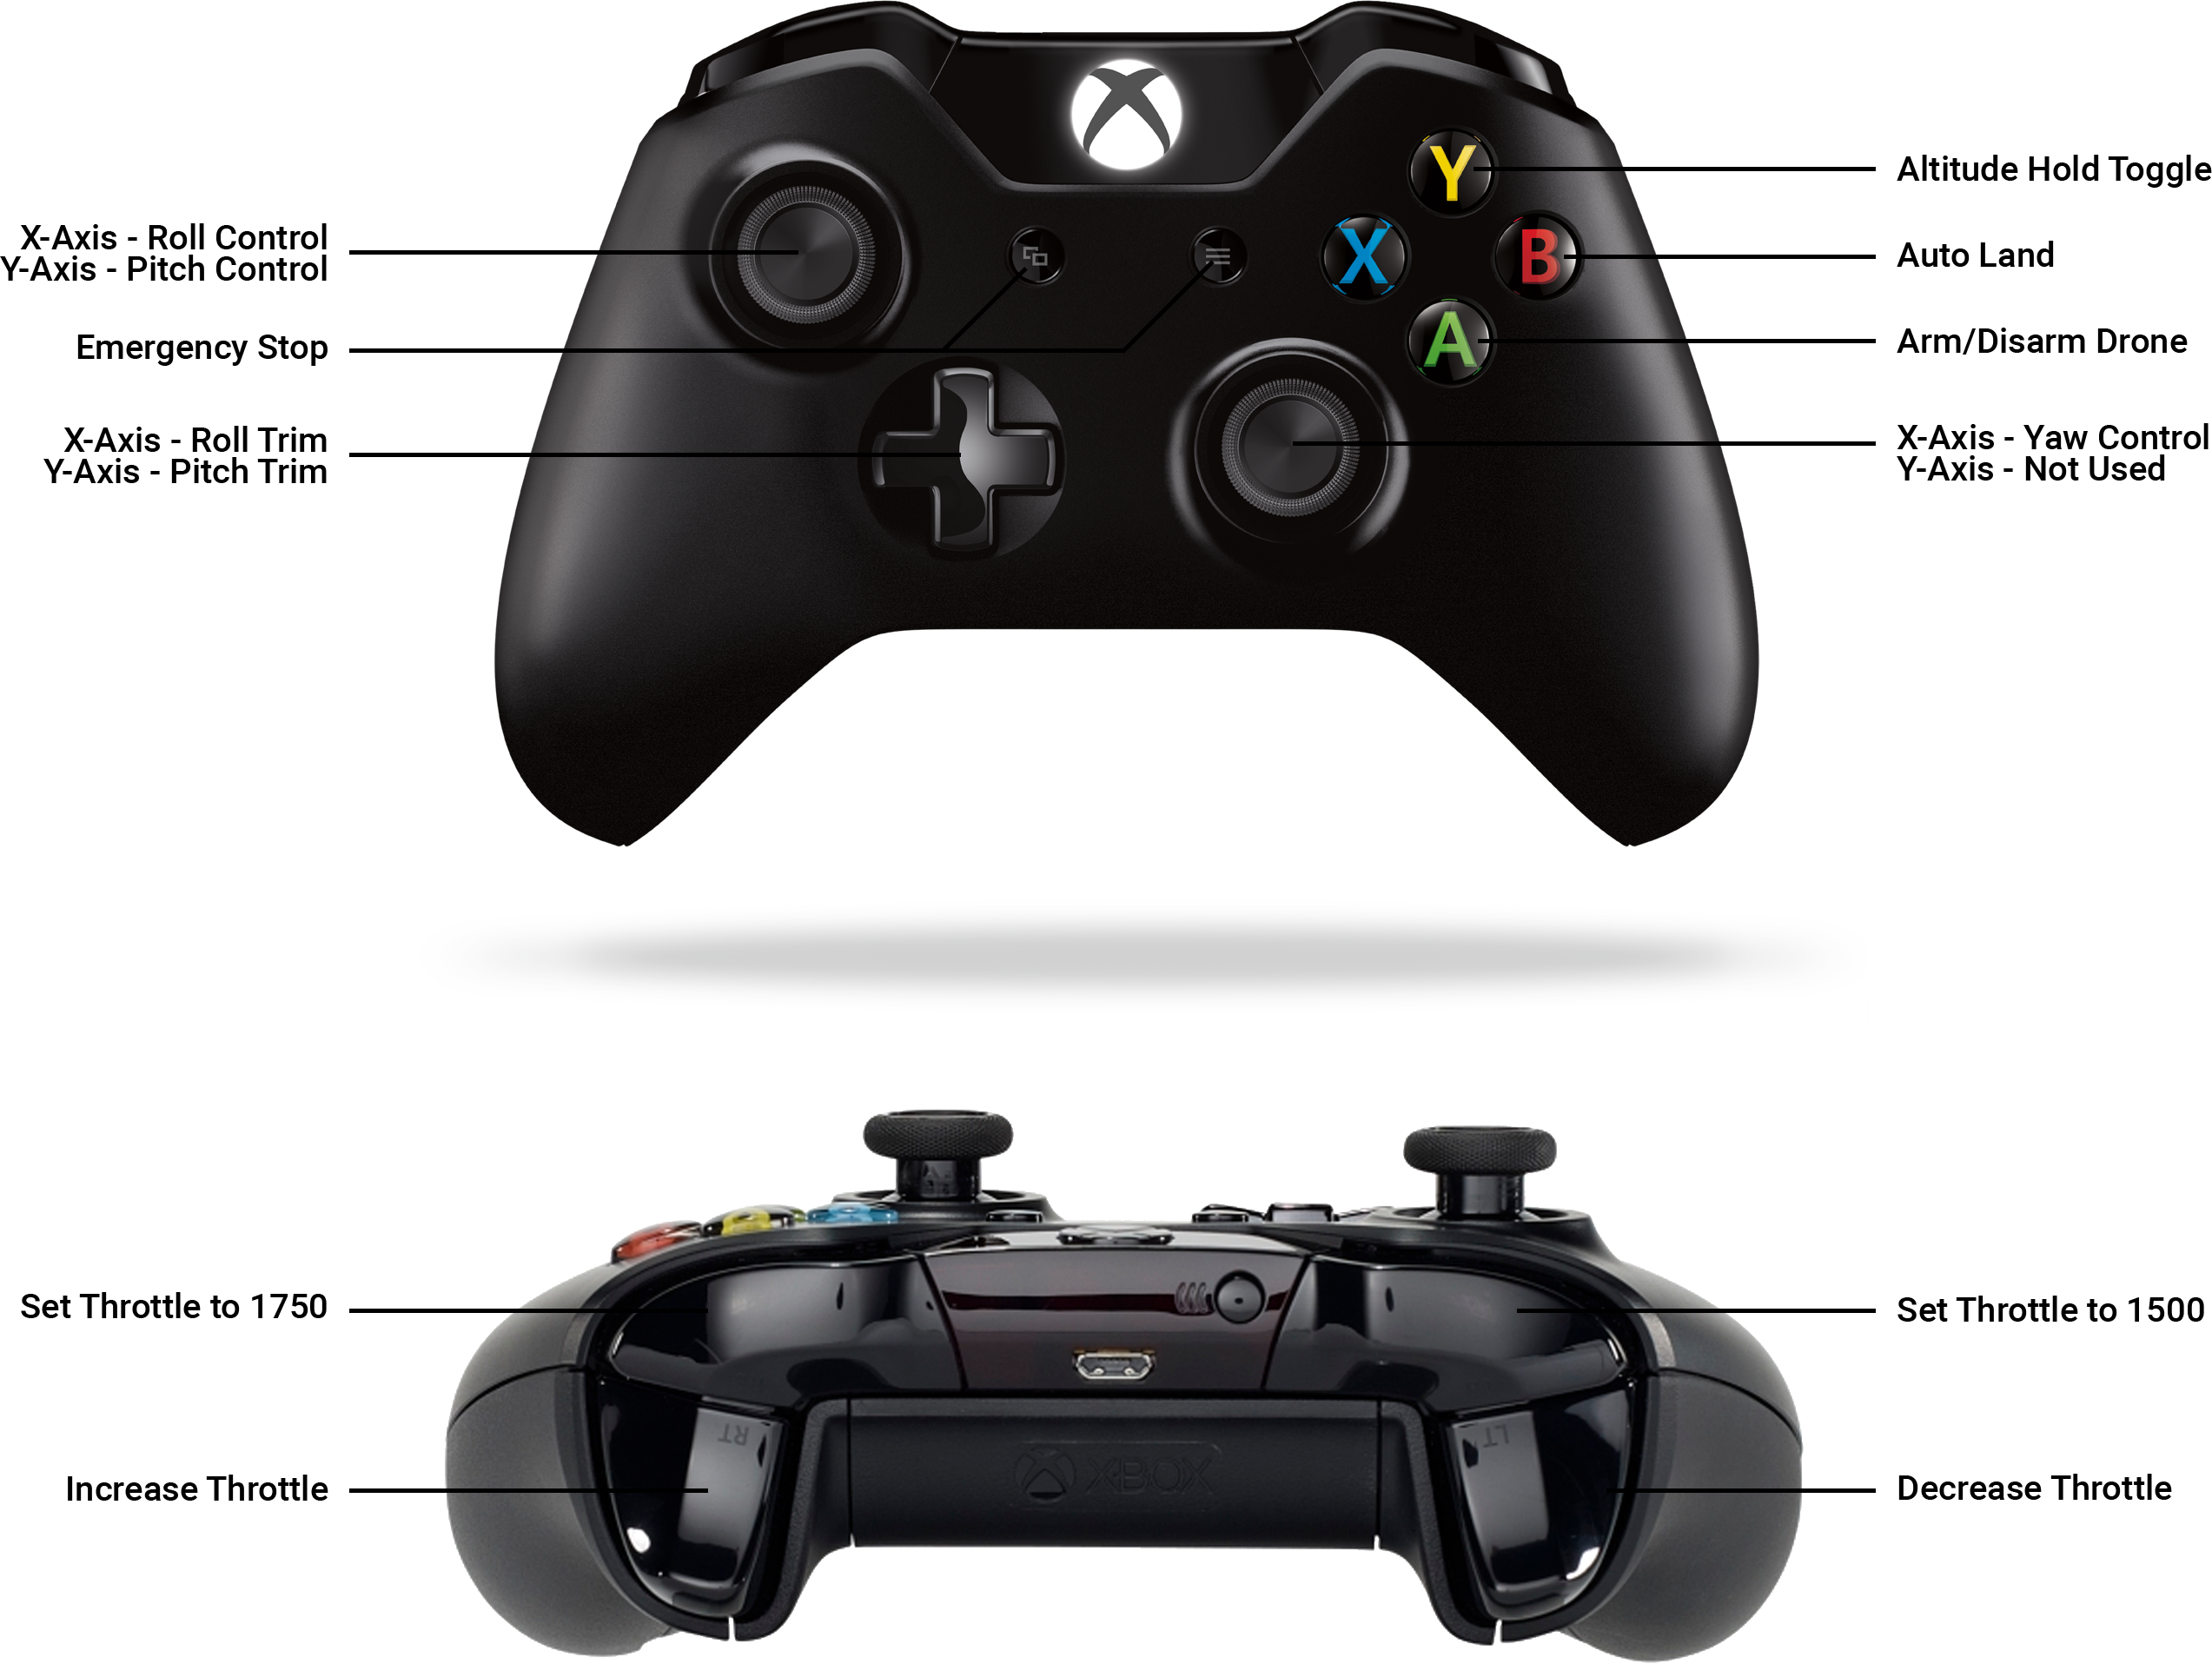
\includegraphics[width=\textwidth]{images/joystick_controls}
\caption{Labeled diagram showing the mapping of the different controls on the Xbox\textsuperscript{\textregistered} One Controller\cite{xbox}}
\label{fig:joycon}
\end{figure}

\bigskip

\begin{itemize}
\item \textbf{Throttle} | \textit{Range: 1000 - 2000} | This sets the base throttle value for all the motors in manual control mode and is used to control the altitude set point in auto flight mode.\\

\item \textbf{Roll} | \textit{Range: -60 - +60} | This channel varies the set point for the roll angle to maneuver the drone in the left-right direction.\\

\item \textbf{Pitch} | \textit{Range: -60 - +60} | This channel varies the set point for the pitch angle to maneuver the drone in the left-right direction.\\

\item \textbf{Yaw} | \textit{Range: -180 - +180} | This channel varies the set point for the yaw angle rotate the drone either in the clockwise or anti-clockwise direction.\\

\item \textbf{Arm} | \textit{Range: 0 or 2000 on AUX1} | Initially, when the drone in switched on, the motors must be disabled for safety. When the drone is ready for flight, the pilot must enable the motors and this is referred to as Arming the drone.\\

\item \textbf{Altitude Hold} | \textit{Range: 0 or 2000 on AUX2} | This control toggles between manual and auto flight modes. In manual flight mode, the user is responsible for maintaining the altitude by varying the throttle. In auto mode, the drone will hold its current altitude.\\

\item \textbf{Pitch Trim} | \textit{Range: Increments of $\pm$0.4 on AUX3} | Adds an offset angle to the pitch axis so that drone is perfectly balanced about this axis.\\

\item \textbf{Roll Trim} | \textit{Range: Increments of $\pm$0.4 on AUX4} | Adds an offset angle to the roll axis so that drone is perfectly balanced about this axis.\\

\item \textbf{Emergency Stop} | \textit{Range: None} | Immediately disarms the drone and resets all the other controls. Note that the same button is used to terminate the communication and close the COM port.

\end{itemize}

\clearpage

\section{Interfacing in Python}
The \textit{pygame.joystick} module manages the joystick devices on a computer. Joystick devices include trackballs and video-game-style gamepads, and the module allows the use of multiple \textit{buttons} and \textit{hats}. The complete documentation and usage of this module can be found \href{https://www.pygame.org/docs/ref/joystick.html}{here}. First, we have to initialize the joystick module as follows.\\

\begin{minted}[linenos=true]{python}
pygame.init()
j = pygame.joystick.Joystick(0)
j.init()
\end{minted}

\bigskip

The Joystick object allows you to get information about the types of controls on a joystick device. Once the device is initialized the pygame event queue will start receiving events about its input. Pygame handles all its event messaging through an event queue. \href{https://www.pygame.org/docs/ref/event.html#pygame.event.pump}{\textit{pygame.event.pump()}} handles all this for us. In the program loop, we to make some sort of call to the event queue \textit{(line 4)}.\\

Now, we can read all the data from the controller as shown below. The \textit{get{\_}numaxes()} and \textit{get{\_}numbuttons()} methods return the number of joystick axes and buttons on the controller respectively.\\

\begin{minted}[linenos=true]{python}
def getJoystick():
    out = [0]*5 + [0]*10 + [0] # List to store output data
    it = 0 # Iterator
    
    # Handle event queue
    pygame.event.pump()
    
    # Read input from the analog sticks       
    for i in range(0, j.get_numaxes()):
        out[it] = j.get_axis(i)
        it += 1
        
    # Read input from buttons
    for i in range(0, j.get_numbuttons()):
        out[it] = j.get_button(i)
        it += 1
	
    # Read input from the hat (D-pad)
    out[it] = j.get_hat(0)
    
    # Return the data 
    return out
\end{minted}

\bigskip

The analog stick axes data are floating point values ranging from -1 to +1. The button outputs are digital values (0 or 1). The \href{https://en.wikipedia.org/wiki/D-pad}{hat} values are ($\pm1$) for both the axes.\\

Now that we have the data from the controller, we have to send it to the quadcopter in a format that it understands. We will use the MultiWii Serial Protocol. The \textit{MultiWii.py} provides methods to send frames serially over a COM port. The tutorial of working of MSP is already covered. In Python, we can store the data payload in the form of a list and use the \textit{struct.pack()} method to convert our payload into a byte array. The packing formats are explained \href{https://docs.python.org/2/library/struct.html#format-characters}{here}. Create a new MultiWii object and initialize the COM port as follows.\\

\begin{minted}[linenos=true]{python}
from MultiWii import *

drone = MultiWii()
drone.start('COM10') # Virtual COM port number
\end{minted}
\bigskip

We have to now convert the controller data to scale it to ranges as given in \textit{\autoref{sec:loc}}. Note that these ranges are not standard MSP ranges and have been modified as per our requirement. The user can send any custom data on the auxiliary channels. We will use the \textit{MSP{\_}SET{\_}RAW{\_}RC} frame to send our control data. The following is a simple example to do this.\\

\begin{minted}[linenos=true]{python}
# List to store converted MSP data to be sent
set_raw_rc = [0, 0, 0, 0, 0, 0, 0, 0]

# Get the input data from the controller
js = getJoystick()

# Increase/Decrease throttle
set_raw_rc[0] = int(constrain(set_raw_rc[0] + (js[2])/3.0), 1000, 2000))

# Roll angle
set_raw_rc[1] = int(js[1] * 60)

# Pitch angle
set_raw_rc[2] = int(js[0] * 60) # Multiply by -60 if axis is inverted

# Yaw angle
set_raw_rc[3] = int(js[4] * 180)

# AUX1 - Arm drone button
set_raw_rc[4] = js[5] * 2000

# AUX2 - Altitude hold button
set_raw_rc[5] = js[8] * 2000

# Pack eight INT8 elements and send the frame
drone.sendFrame(drone.SET_RAW_RC, set_raw_rc, '<8h')

# Delay for 100ms
time.sleep(0.1)
\end{minted}

\bigskip

Run the above snippet in your program loop (\href{https://www.youtube.com/watch?v=NIWwJbo-9_8}{\textit{try-except}} in a \textit{while} loop recommended). Finally, before your program ends, make sure you close the COM port and uninitialize the joystick module as follows to prevent the program from hanging.\\

\begin{minted}[linenos=true]{python}
pygame.quit()
drone.close()
\end{minted}

\bigskip

The above snippet is just a simple example. You can implement your own controls. The controls can also be made \textit{sticky}, where the joystick axis is used only to increase or decrease values, instead of giving the absolute value of the joystick position. You can even make the \href{https://stackoverflow.com/questions/19749404/is-it-possible-to-rumble-a-xbox-360-controller-with-python}{joystick controller vibrate} for user feedback, if your controller supports it. A CLI in Python was developed to visualize the joystick controls as shown in \textit{\autoref{fig:xbox_cli}}. This is the \textit{link} for the video demonstration of the joystick controller interfaced with it.\\

\begin{figure}[!htb]
\centering
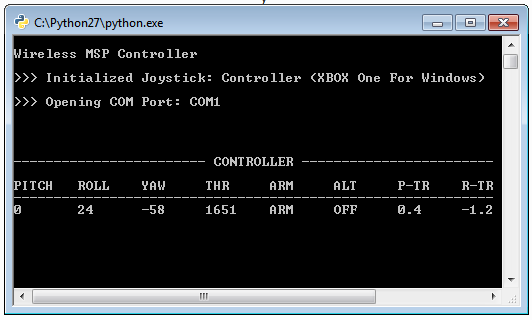
\includegraphics[width=\textwidth]{images/xbox_cli}
\caption{A CLI developed in Python for the wireless joystick controller}
\label{fig:xbox_cli}
\end{figure}



\begin{thebibliography}{20}
%\addcontentsline{toc}{chapter}{References}

\bibitem{xbox}
Xbox\textsuperscript{\textregistered} One is a trademark of Microsoft Corporation. The Xbox\textsuperscript{\textregistered} Logos are trademarks of Microsoft\textsuperscript{\textregistered} Corporation.

\end{thebibliography}

%-------------------------------------------------------------------

\end{document}

